\documentclass[12pt]{article}
\usepackage{amsmath}
\usepackage{graphicx}
\title{Report for Auto Control Lab9}
\date{2020/11/17}
\author{Jacky Yeh 4107064003}

\begin{document}
\begin{titlepage}

\maketitle
\end{titlepage}


\section{Introduction}
This is the eleventh Experiment of Auto Control Lab where TAs taught us the plot of more characteristics of the system which includes which includes percentage overshoot, and more precise system plots.


\section{LAB9}
\subsection{Part 1 Homework problems and its codes}
Objective:To perform operations to find out the response of the feedback system of a given time interval\\

These are the stated Homework problems\\

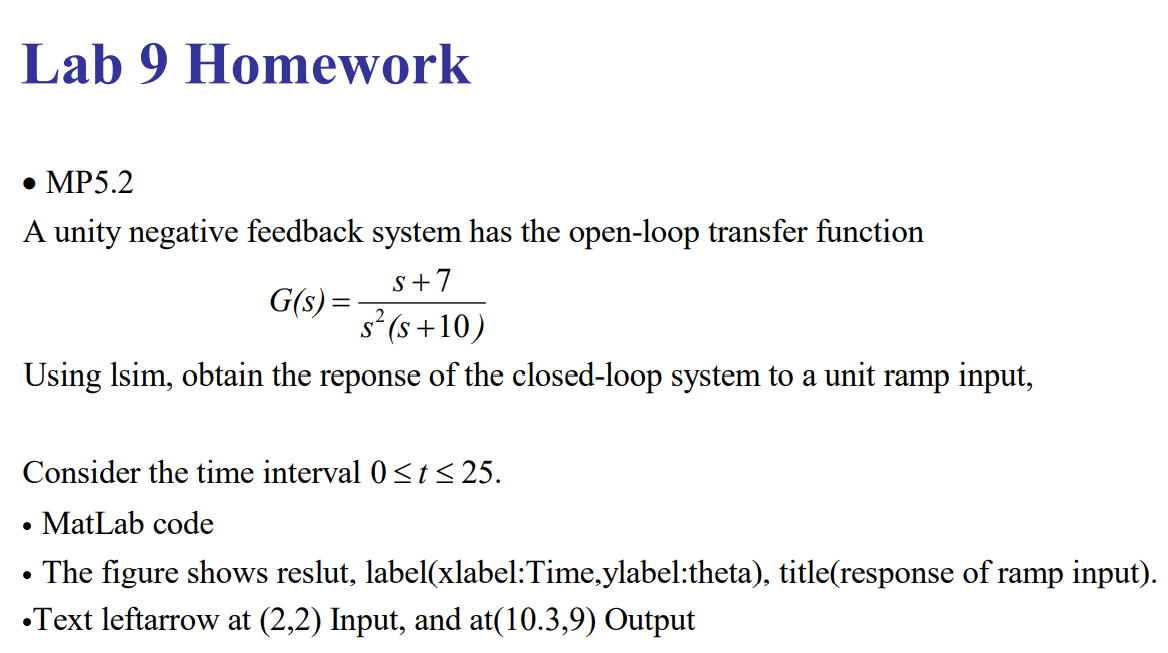
\includegraphics[scale=0.5]{../Lab9/Pictures/hw1.png} \\

\cleardoublepage

\subsection{CODES FOR PROBLEM1}
In order to perform the tasks, Matlab codes are needed. The following is the code needed for plotting\\

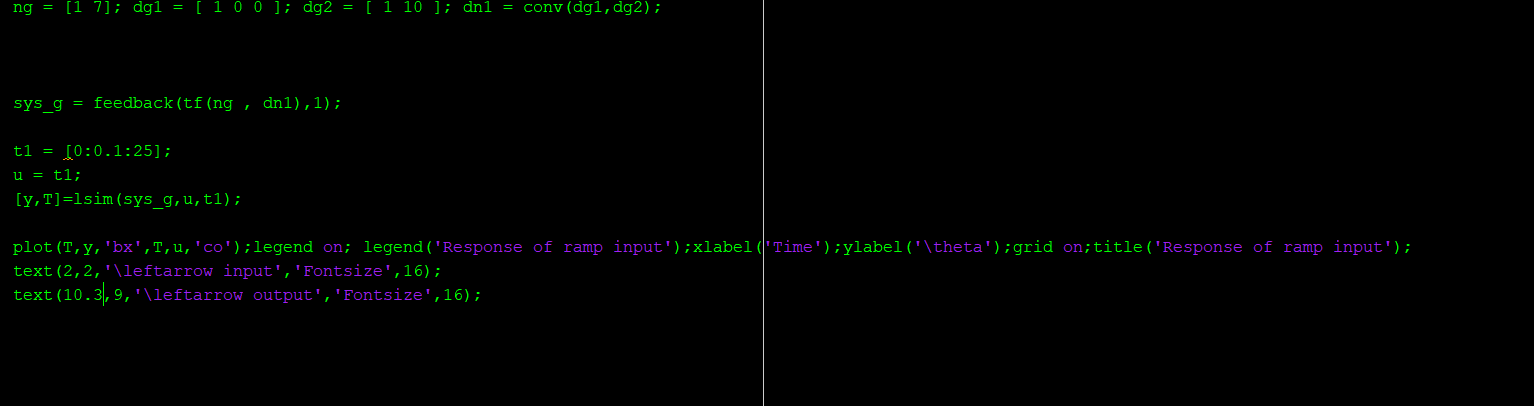
\includegraphics[scale=0.5]{../Lab9/Pictures/code1.png}  \\ 

\subsection{Result of the given system's plot} 

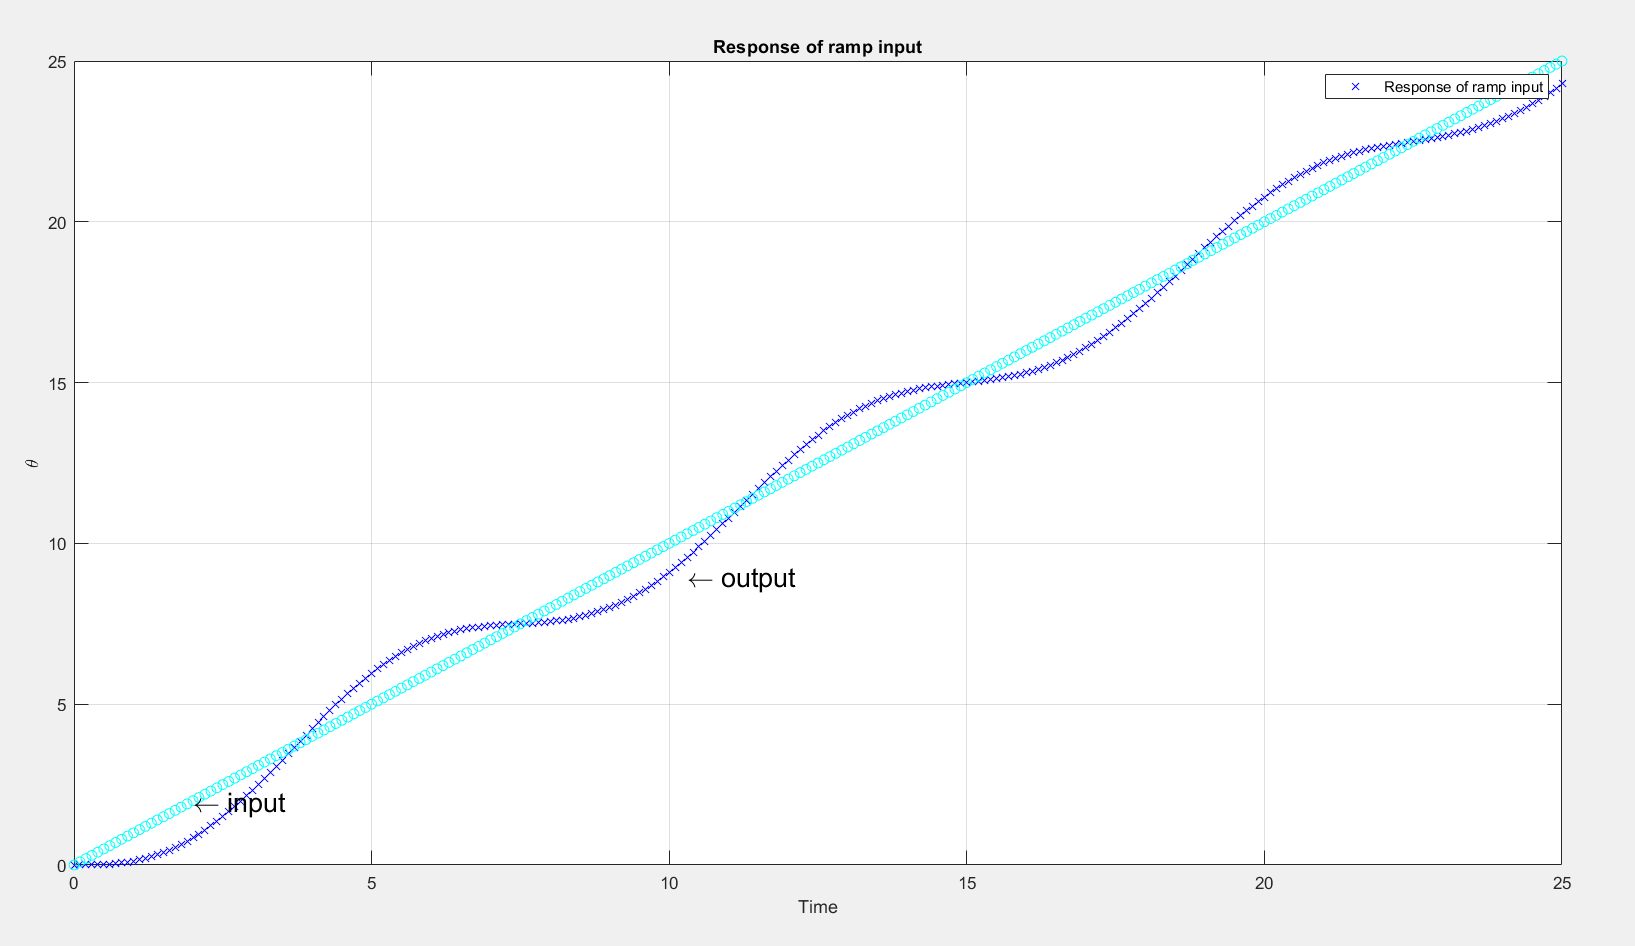
\includegraphics[scale=0.5]{../Lab9/Pictures/output1.png}  \\ 


\cleardoublepage



 
\cleardoublepage
\subsection{Part 2 Homework problems and its codes}
Objective:To plug in and plot out the response with the given 2nd order system to an impulse response. We here needs different system response with different damping ratio $w_{n}$ and natural frequency $\zeta$

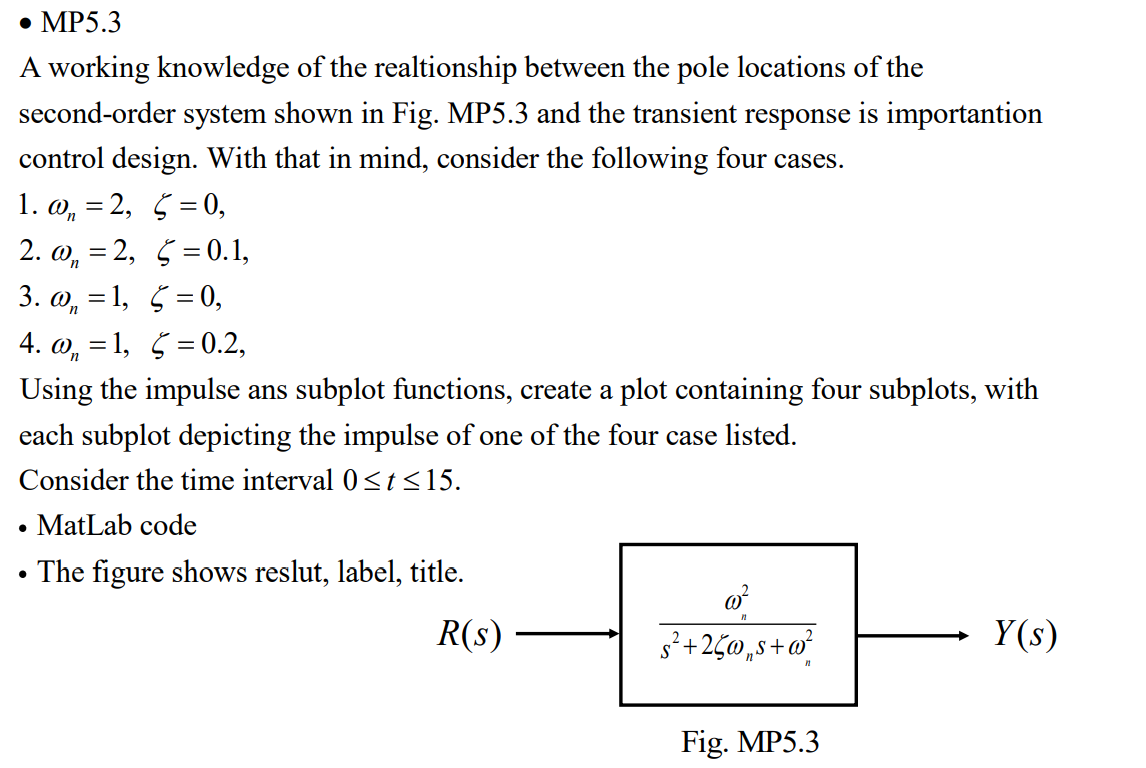
\includegraphics[scale=0.5]{../Lab9/Pictures/hw2.png}  \\



\subsection{CODES FOR Part2}
In order to perform the tasks, Matlab codes are needed. The following code is used for plotting the system with different damping ratios and natural frequency \\

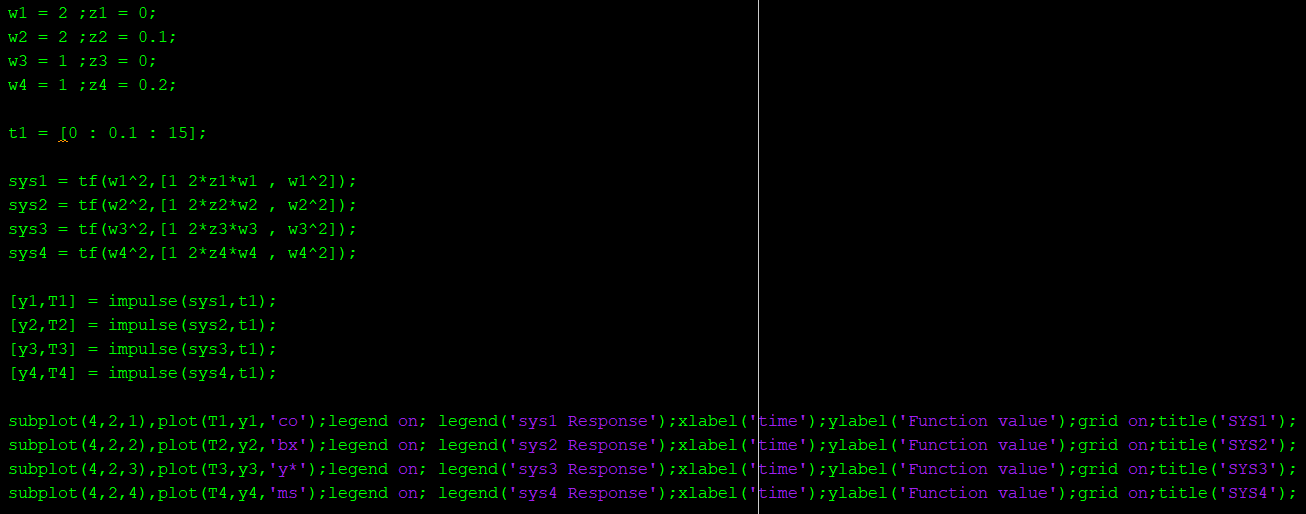
\includegraphics[scale=0.42]{../Lab9/Pictures/code2.png} 


\subsection{Plot Response OF the given systems with different $\zeta$ and $w_{n}$} 
The following is the systems out given\\

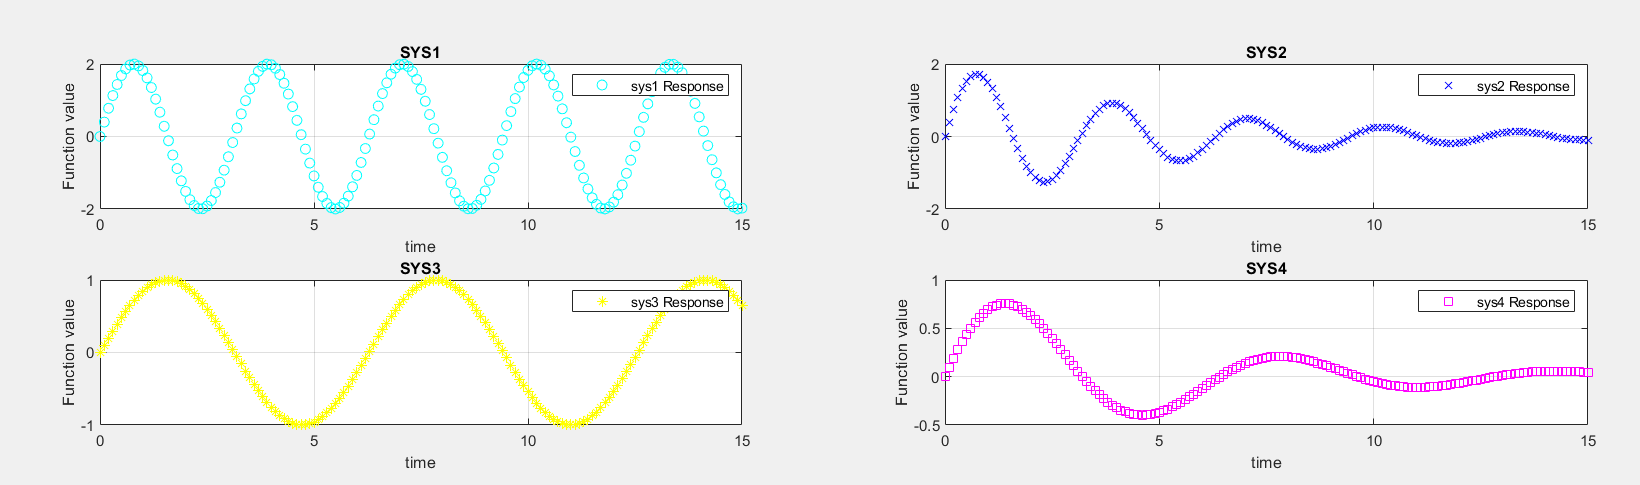
\includegraphics[scale=0.5]{../Lab9/Pictures/output2.png}  \\


\subsection{Part 3 Homework problems and its codes}
Objective:To plug in and plot out the response for impulse responses using lsim function

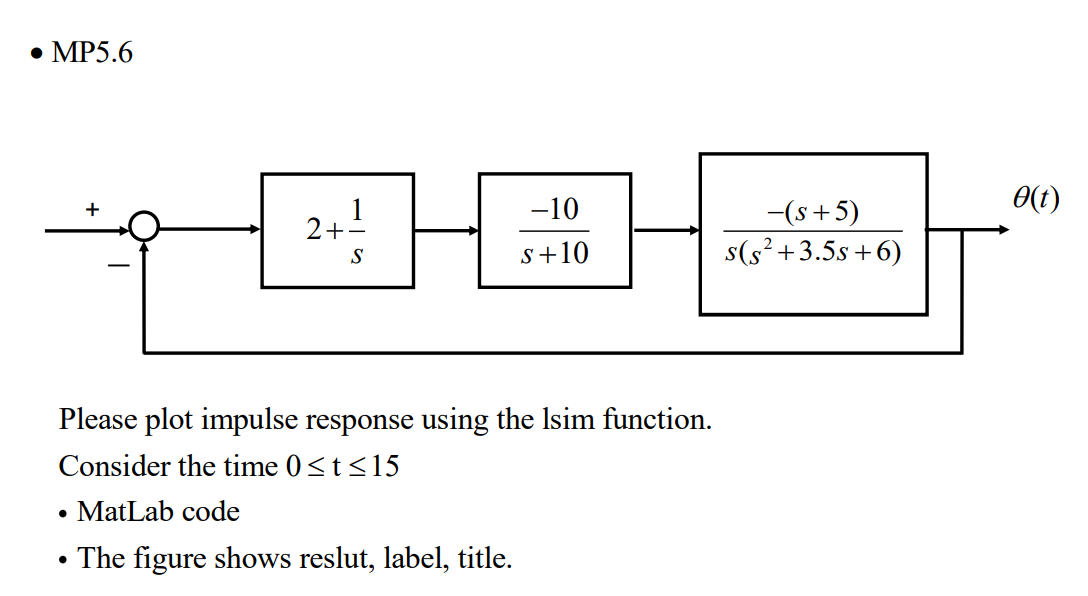
\includegraphics[scale=0.5]{../Lab9/Pictures/hw3.png} 



\subsection{CODES FOR Part3}
In order to perform the tasks, Matlab codes are needed. The following code is used for plotting the system \\

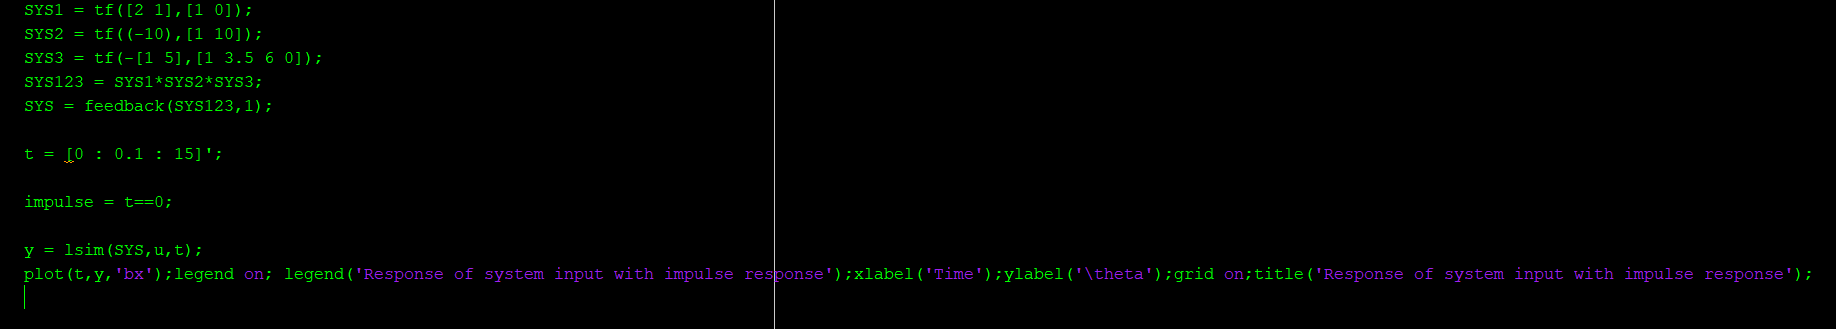
\includegraphics[scale=0.5]{../Lab9/Pictures/code3.png} \\


\subsection{Plot of the system} 
The following is the system out given\\

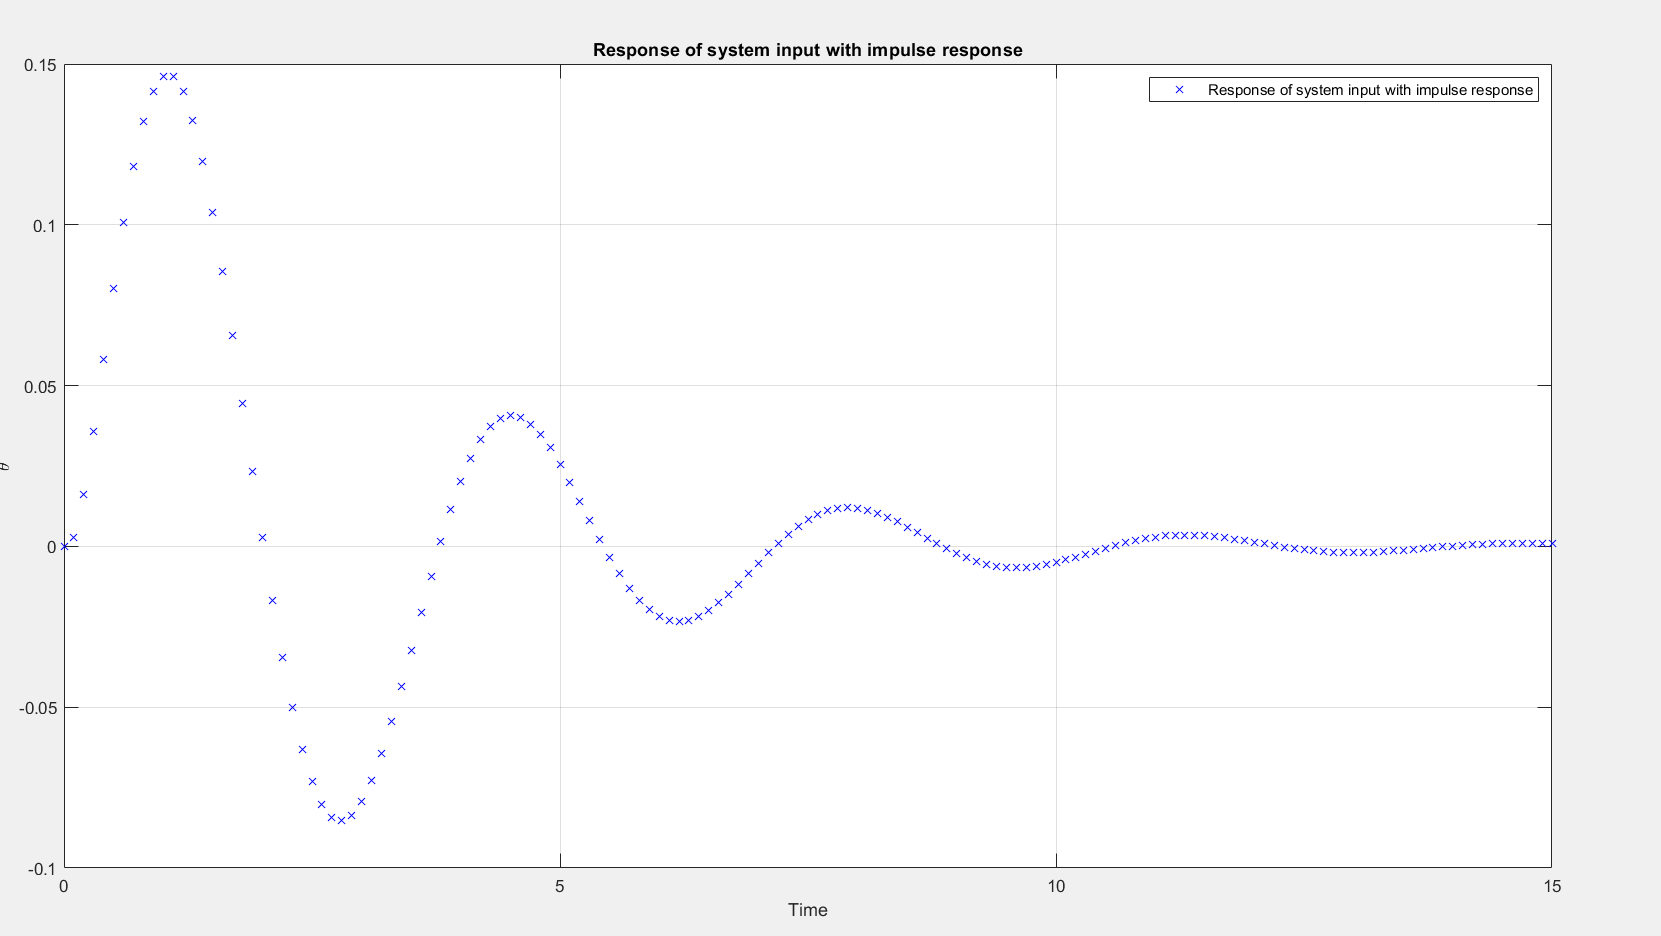
\includegraphics[scale=0.4]{../Lab9/Pictures/output3.png}  \\




\section{Conclusion}
Today we learn how to plot more system response using the techniques we just used. And add more details to the system plots including more labels, results and titles. Also more characteristics for the response like percent overshoot, settling time, peak time and others more. Reviewing what I've just learnt in the Auto Control course.

\begin{center} 
This concludes the eleventh Week of Auto Control LAB\\
\end{center}

\end{document} 
